
% !TEX encoding = UTF-8 Unicode



\documentclass[a4paper]{article}
\usepackage{dirtytalk}
\usepackage{geometry}
\geometry{
 a4paper,
 total={150mm,247mm},
 left=30mm,
 top=30mm,
 }
\usepackage{quotchap}

\usepackage{graphicx}
\usepackage{epstopdf}
\DeclareGraphicsExtensions{.eps}
\usepackage{url}
\usepackage{multicol}% http://ctan.org/pkg/multicols
\usepackage{epigraph}
\setlength{\epigraphwidth}{.85\textwidth}

\usepackage[utf8x]{inputenc} 

\usepackage{array}
\newcolumntype{L}[1]{>{\raggedright\let\newline\\\arraybackslash\hspace{0pt}}m{#1}}
\newcolumntype{C}[1]{>{\centering\let\newline\\\arraybackslash\hspace{0pt}}m{#1}}
\newcolumntype{R}[1]{>{\raggedleft\let\newline\\\arraybackslash\hspace{0pt}}m{#1}}
\usepackage{subcaption}
\usepackage[utf8]{inputenc}
\usepackage[portuguese]{babel}
\usepackage{listings,mdframed}

\usepackage{textcomp}
\usepackage{hyperref}

\usepackage{float}
\usepackage{listings}

\lstdefinestyle{esc} {
language=c,
	keywordstyle=\bfseries\ttfamily\color[rgb]{0,0,1},
	identifierstyle=\ttfamily,
	commentstyle=\color[rgb]{0.133,0.545,0.133},
	stringstyle=\ttfamily\color[rgb]{0.627,0.126,0.941},
	showstringspaces=false,
	basicstyle=\tiny,
numberstyle=\small,
numbers=right,
	stepnumber=1,
	numbersep=10pt,
	tabsize=1,
	breaklines=true,
	prebreak = \raisebox{0ex}[0ex][0ex]{\ensuremath{\hookleftarrow}},
	breakatwhitespace=false,
	%aboveskip={1.5\baselineskip},
  columns=fixed,
  upquote=true,
  extendedchars=true,
 frame=single,
}

\lstdefinestyle{command}{
backgroundcolor=\color{yellow},frame=shadowbox,
language=c,
	keywordstyle=\bfseries\ttfamily\color[rgb]{0,0,1},
	identifierstyle=\ttfamily,
	commentstyle=\color[rgb]{0.133,0.545,0.133},
	stringstyle=\ttfamily\color[rgb]{0.627,0.126,0.941},
	showstringspaces=false,
	basicstyle=\small,
numberstyle=\small,
numbers=right,
	stepnumber=1,
	numbersep=10pt,
	tabsize=1,
	breaklines=true,
	prebreak = \raisebox{0ex}[0ex][0ex]{\ensuremath{\hookleftarrow}},
	breakatwhitespace=false,
	%aboveskip={1.5\baselineskip},
  columns=fixed,
  upquote=true,
  extendedchars=true,
}

\lstset{
	language=c,
	keywordstyle=\bfseries\ttfamily\color[rgb]{0,0,1},
	identifierstyle=\ttfamily,
	commentstyle=\color[rgb]{0.133,0.545,0.133},
	stringstyle=\ttfamily\color[rgb]{0.627,0.126,0.941},
	showstringspaces=false,
	basicstyle=\small,
numberstyle=\small,
numbers=right,
	stepnumber=1,
	numbersep=10pt,
	tabsize=1,
	breaklines=true,
	prebreak = \raisebox{0ex}[0ex][0ex]{\ensuremath{\hookleftarrow}},
	breakatwhitespace=false,
	%aboveskip={1.5\baselineskip},
  columns=fixed,
  upquote=true,
  extendedchars=true,
 frame=single
 %backgroundcolor=\color{lbcolor},
}

\usepackage{titling}
\newcommand{\subtitle}[1]{%
  \posttitle{%
    \par\end{center}
    \begin{center}\large#1\end{center}
    \vskip0.5em}%
}


\begin{document}
\title{Performance e Precisão Relativas de Filesystem Benchmarks e Disk Benchmarks}

\subtitle{Active Benchmarking da ferramenta iozone recorrendo a DTrace em Solaris 11}

% author names and affiliations
% use a multiple column layout for up to three different
% affiliations
\author{{Filipe Oliveira}
Departamento de Informática\\
Universidade do Minho\\
Email: a57816@alunos.uminho.pt}
}



% make the title area
\maketitle

% As a general rule, do not put math, special symbols or citations
% in the abstract
%\begin{abstract}

%Neste estudo, analisamos a performance de kernels 
%\end{abstract}

% no keywords




% For peer review papers, you can put extra information on the cover
% page as needed:
% \ifCLASSOPTIONpeerreview
% \begin{center} \bfseries EDICS Category: 3-BBND \end{center}
% \fi
%
% For peerreview papers, this IEEEtran command inserts a page break and
% creates the second title. It will be ignored for other modes.



%\section{Introduction}
% no \IEEEPARstart
%This demo file is intended to serve as a ``starter file''
%for IEEE Computer Society conference papers produced under \LaTeX\ using
%IEEEtran.cls version 1.8b and later.
% You must have at least 2 lines in the paragraph with the drop letter
% (should never be an issue)
%I wish you the best of success.

%\hfill Filipe Oliveira
 
%\hfill 1 Março, 2016
\renewcommand{\abstract}{\textbf{\centering Introdução -- Contextualização da Ferramenta iozone\break}}

\abstract{

A necessidade de recurso a ferramentas de Benchmarking está implicitamente associada à necessidade de recolha de informação dos sistemas de computação no seu todo, ou de pontos específicos do mesmo, e sua posterior comparação e interpretação. Ora, quando queremos estudar especificamente a performance de um sistema de ficheiros e/ou de um determinado tipo de dispositivo de armazenamento de informação, podemos recorrer a ferramentas de traçado dinâmico (como o dtrace) por forma a confirmar os resultados obtidos e/ou complementar os mesmos, de uma forma que outrora era de extrema complexidade e dificuldade. \par 
É importante realçar que a performance relativa dos sistemas de ficheiros e dispositivos de armazenamento está implicitamente ligada, uma vez que através de caching, buffering, e I/O assíncrono um sistema de ficheiros poderá "esconder" do nível da aplicação determinadas propriedades e lacunas do dispositivo físico de armazenamento. Retornando às ferramentas de benchmarking de sistemas de ficheiros e/ou dispositivos de armazenamento podemos compreender que as técnicas de software/hardware de otimização de tempos acesso aos dados, poderão implicar a benchmarking pouco precisa dos sistemas físicos presentes no sistema. \par 
Todos os métodos de redução de tempos de acesso, ou seja, todos os métodos que tentam esconder a latência de acesso aos dados, deverão ser tidas em contacto no momento do benchmarking. Este trabalho prende-se precisamente com o estudo do quão precisa é a ferramenta de benchmarking iozone em sistemas de computação Solaris based, nomeadamente na máquina descrita na tabela \ref{table:characterization}.


\begin{table}[H]
\caption{Características de Hardware do sistema de computação }
     \label{table:characterization}
\centering
  \begin{tabular}{ | l | r | }
  
    \hline
    Sistema & compute-641 \\ \hline \hline
        \# CPUs & 2  \\ \hline
    CPU & Intel\textsuperscript{\textregistered} Xeon\textsuperscript{\textregistered}  E5-2650 v2 \\ \hline 
    Arquitectura de Processador & Ivy Bridge  \\ \hline 
    \# Cores por CPU & 8   \\ \hline 
    \# Threads por CPU & 16  \\ \hline 
     Freq. Clock & 2.6 GHz  \\ \hline
    Cache L1  & 256KB  (32KB por Core)  \\ \hline 
    Cache L2  & 2048KB (256KB por Core)  \\ \hline 
    Cache L3  & 20480KB (partilhada) \\ \hline 
  Ext. Inst. Set  & SSE4.2, AVX  \\ \hline 
         \#Memory Channels & 4 \\ \hline
        Memória Ram Disponível & 64GB \\ \hline
     Peak Memory BW Fab. CPU  & 59.7 GB/s \\ \hline
     \textbf{Local FileSystems} & ufs \\ \hline
    \textbf{ NFS FileSystems} & nfs,
smb, 
autofs, 
smbfs\\ \hline
  \end{tabular}
\end{table}

Aquando da realização de benchmarking via iozone, iremos recorrer a outras ferramentas (nomeadamente truss e dtrace) para procedermos à nossa própria benchmark -- vulgo Active Benchmarking. Pretendemos com isso determinar quais os principais "bottlenecks" da porção do sistema a analisar, e ao mesmo tempo desenvolver capacidade crítica na análise de dados relativos a performance de sistemas de computação de complexidade acrescida.\par 
Precisamos primeiramente de analisar de uma forma geral o comportamento da aplicação iozone no que  concerne a system calls, traçando de seguida um plano de traçado dinâmico que corrobore/desminta o apresentado pela ferramenta. 
I
\section{Passive Benchmarking :: uma primeira análise à ferramenta}

Definida a ferramenta de benchmarking - iozone - existem diferentes opções a ter em conta, nomeadamente:
\begin{itemize}
\item tipo de operação -- read, write, re-read, re-write, e outros
\item tamanho do I/O
\item forma de acesso aos dados -- sequencial ou random
\item Memory mapping -- acesso á memória mmap em detrimento de read/write.
\end{itemize}
Teremos que ter ainda em conta na escolha do tamanho do dataset a memória disponível, assim como a quantidade dados passíveis de estarem presentes na memória cache. Só assim conseguiremos garantir que o recurso a uma system call irá resultar numa leitura/escrita em disco, ultrapassando os vários níveis de disfarce de latência.\par 
Ora, dado que é na escrita dos dados que acreditamos que existirá uma maior possibilidade de descrepância de resultados pelo iozone versus os que iremos obter por medição direta (dados os inúmeros mecanismos como caching, buffering, e I/O assíncrono, permitirem a uma kernel efectuar uma escrita sem necessariamente os dados serem imediatamente escritos no disco), tomaremos especial atenção à performance de escrita medida pela ferramenta.\par 
Ora, e atendendo ao seguinte excerto das Iozone Run rules:

\epigraph{\textbf{For disk performance comparisons:}\par 
1. For single stream results, be sure the file size is 3 times the size of the buffer cache. For throughput results, be sure the aggregate of files is 3 times the size of the buffer cache.\\\url{}}

Daqui retiramos que o tamanho do ficheiro deverá ser 3 vezes superior à buffer cache disponível nos sistema de computação. Precisamos portanto de determinar esse valor, dado pelo parâmetro \textbf{UFS bufhwm}. Atente na sua descrição:

\epigraph{\textbf{UFS Parameters}\\
\textbf{bufhwm and bufhwm\_pct}\\
\textbf{Description:}\par 

Defines the maximum amount of memory for caching I/O buffers. The buffers are used for writing file system metadata (superblocks, inodes, indirect blocks, and directories). Buffers are allocated as needed until the amount of memory (in KB) to be allocated exceed bufhwm. At this point, metadata is purged from the buffer cache until enough buffers are reclaimed to satisfy the request.
\vspace{3mm}\\ \url{http://docs.oracle.com/cd/E23823_01/html/817-0404/chapter2-37.html}}

Ora, recorrendo ao comando \textbf{sysdef} podemos extrair a informação desejada:

\begin{lstlisting}[style=command]
 sysdef
 ...
*
* Tunable Parameters
*
1373298688	maximum memory allowed in buffer cache (bufhwm)
...
   \end{lstlisting}
   
Poderíamos ser induzidos em erro e considerar como 3 * 1373298688 KB o tamanho do ficheiro a utilizar. Contudo, um olhar mais atento à continuação da definição de \textbf{bufhwm}:
\epigraph{


\textbf{Range}\\ 
80 KB to 20 percent of physical memory, or 2 TB, whichever is less. Consequently, bufhwm\_pct can be between 1 and 20.\\

\textbf{Validation}\\
If bufhwm is less than its lower limit of 80 KB or \textbf{greater than its upper limit} (the lesser of 20 percent of physical memory, 2 TB, or one quarter (1/4) of the maximum amount of kernel heap), it is reset to the upper limit. The following message appears on the system console and in the /var/adm/messages file if an invalid value is attempted:
\vspace{3mm}\\ \url{http://docs.oracle.com/cd/E23823_01/html/817-0404/chapter2-37.html}}\par 
leva-nos a calcular o valor máximo de bufhwm como ( 20\% de 65501000 KB )  * 3 =  39300600 KB = 39.3006 GB. 
\par 

\subsection{Command Line Options}
Analisando ainda as \say{Command Line Options} da ferramenta podemos desde já enumerar algumas opções que devemos incluir:

\begin{itemize}
\item \textbf{ -i 0 } -- Used to specify which tests to run. (0=write/rewrite, 1=read/re-read, 2=random-read/write 3=Read-backwards, 4=Re-write-record, 5=stride-read, 6=fwrite/re-fwrite, 7=fread/Re-fread, 8=random mix, 9=pwrite/Re-pwrite, 10=pread/Re-pread, 11=pwritev/Re-pwritev, 12=preadv/Re- preadv).

\item \textbf{-s 39g} -- Used to specify the size, in Kbytes, of the file to test. One may also specify -s #k (size in Kbytes) or -s #m (size in Mbytes) or -s #g (size in Gbytes). 

\item \textbf{-S 20480} -- Set processor cache size to value (in Kbytes). This tells Iozone the size of the processor cache. It is used internally for buffer alignment and for the purge functionality.

\item \textbf{-l 1 } -- Set the lower limit on number of processes to run. When running throughput tests this option allows the user to specify the least number of processes or threads to start. This option should be used in conjunction with the -u option.

\item \textbf{-u 1 } -- Set the upper limit on number of processes to run. When running throughput tests this option allows the user to specify the greatest number of processes or threads to start. This option should be used in conjunction with the -l option.

\item \textbf{ -b /export/home/a57816/ESC\_ACTIVE\_BENCHMARKING\_HOME/teste\_write.xls } -- Iozone will create a binary file format file in Excel compatible output of results.

\item \textbf{-R} -- Generate Excel report. Iozone will generate an Excel compatible report to standard out. This file may be imported with Microsoft Excel (space delimited) and used to create a graph of the filesystem performance. Note: The 3D graphs are column oriented. You will need to select this when graphing as the default in Excel is row oriented data.
\end{itemize}

Assim, analisemos resultado  do seguinte comando iozone:
\begin{lstlisting}[style=command]
/opt/csw/bin/iozone -+u -R -i 0 -S 20480 -s 39g -b /export/home/a57816/ESC_ACTIVE_BENCHMARKING_HOME/teste_write.xls -l 1 -u 1 
\end{lstlisting}
   
que apresenta o seguinte resultado:
\begin{lstlisting}
	Iozone: Performance Test of File I/O
	        Version $Revision: 3.434 $
		Compiled for 64 bit mode.
		Build: Solaris10 

	Contributors:William Norcott, Don Capps, Isom Crawford, Kirby Collins
	             Al Slater, Scott Rhine, Mike Wisner, Ken Goss
	             Steve Landherr, Brad Smith, Mark Kelly, Dr. Alain CYR,
	             Randy Dunlap, Mark Montague, Dan Million, Gavin Brebner,
	             Jean-Marc Zucconi, Jeff Blomberg, Benny Halevy, Dave Boone,
	             Erik Habbinga, Kris Strecker, Walter Wong, Joshua Root,
	             Fabrice Bacchella, Zhenghua Xue, Qin Li, Darren Sawyer,
	             Vangel Bojaxhi, Ben England, Vikentsi Lapa,
	             Alexey Skidanov.

	Run began: Mon Apr 18 19:34:12 2016

	CPU utilization Resolution = 0.000 seconds.
	CPU utilization Excel chart enabled
	Excel chart generation enabled
	File size set to 40894464 kB
	Command line used: /opt/csw/bin/iozone -+u -R -i 0 -S 20480 -s 39g -b /export/home/a57816/ESC_ACTIVE_BENCHMARKING_HOME/teste_write.xls -l 1 -u 1
	Output is in kBytes/sec
	Time Resolution = 0.000001 seconds.
	Processor cache size set to 20480 kBytes.
	Processor cache line size set to 32 bytes.
	File stride size set to 17 * record size.
	Min process = 1 
	Max process = 1 
	Throughput test with 1 process
	Each process writes a 40894464 kByte file in 4 kByte records

	Children see throughput for  1 initial writers 	=  489166.09 kB/sec
	Parent sees throughput for  1 initial writers 	=  406767.30 kB/sec
	Min throughput per process 			=  489166.09 kB/sec 
	Max throughput per process 			=  489166.09 kB/sec
	Avg throughput per process 			=  489166.09 kB/sec
	Min xfer 					= 40894464.00 kB
	CPU Utilization: Wall time   83.600    CPU time   77.460    CPU utilization  92.65 %


	Children see throughput for  1 rewriters 	=  463768.00 kB/sec
	Parent sees throughput for  1 rewriters 	=  402978.57 kB/sec
	Min throughput per process 			=  463768.00 kB/sec 
	Max throughput per process 			=  463768.00 kB/sec
	Avg throughput per process 			=  463768.00 kB/sec
	Min xfer 					= 40894464.00 kB
	CPU utilization: Wall time   88.179    CPU time   71.719    CPU utilization  81.33 %




"Throughput report Y-axis is type of test X-axis is number of processes"
"Record size = 4 kBytes "
"Output is in kBytes/sec"

"  Initial write "  489166.09 

"        Rewrite "  463768.00 


"CPU utilization report Y-axis is type of test X-axis is number of processes"
"Record size = 4 kBytes "
"Output is in CPU%"

"  Initial write "      92.65 

"        Rewrite "      81.33 


iozone test complete.
\end{lstlisting}
 
 \subsection{Take 1 -- uma análise com iostat}
Ora, dos resultados anteriores, retiramos que o máximo de throughput do sistema de ficheiros e dispositivo de armazenamento físico tem o valor de 489166.09 KB/s para operações de escrita e 463768.00 KB/s para operações de re-escrita. Este último resultado apresentado leva-nos a duvidar da precisão de medição da ferramenta. Outro indicador que nos leva a duvidar da veracidade da medição prende-se com os valores altíssimos de utilização de CPU time de uma aplicação implicitamente \textbf{IO BOUND}.\par 
Corramos novamente a ferramenta analisando agora o input/output recorrendo à ferramenta \textbf{iostat}, criando uma relação gráfica entre os valores apresentados por ambas as leituras na figura \ref{fig:iostat}.

\begin{figure}[H]
\centering
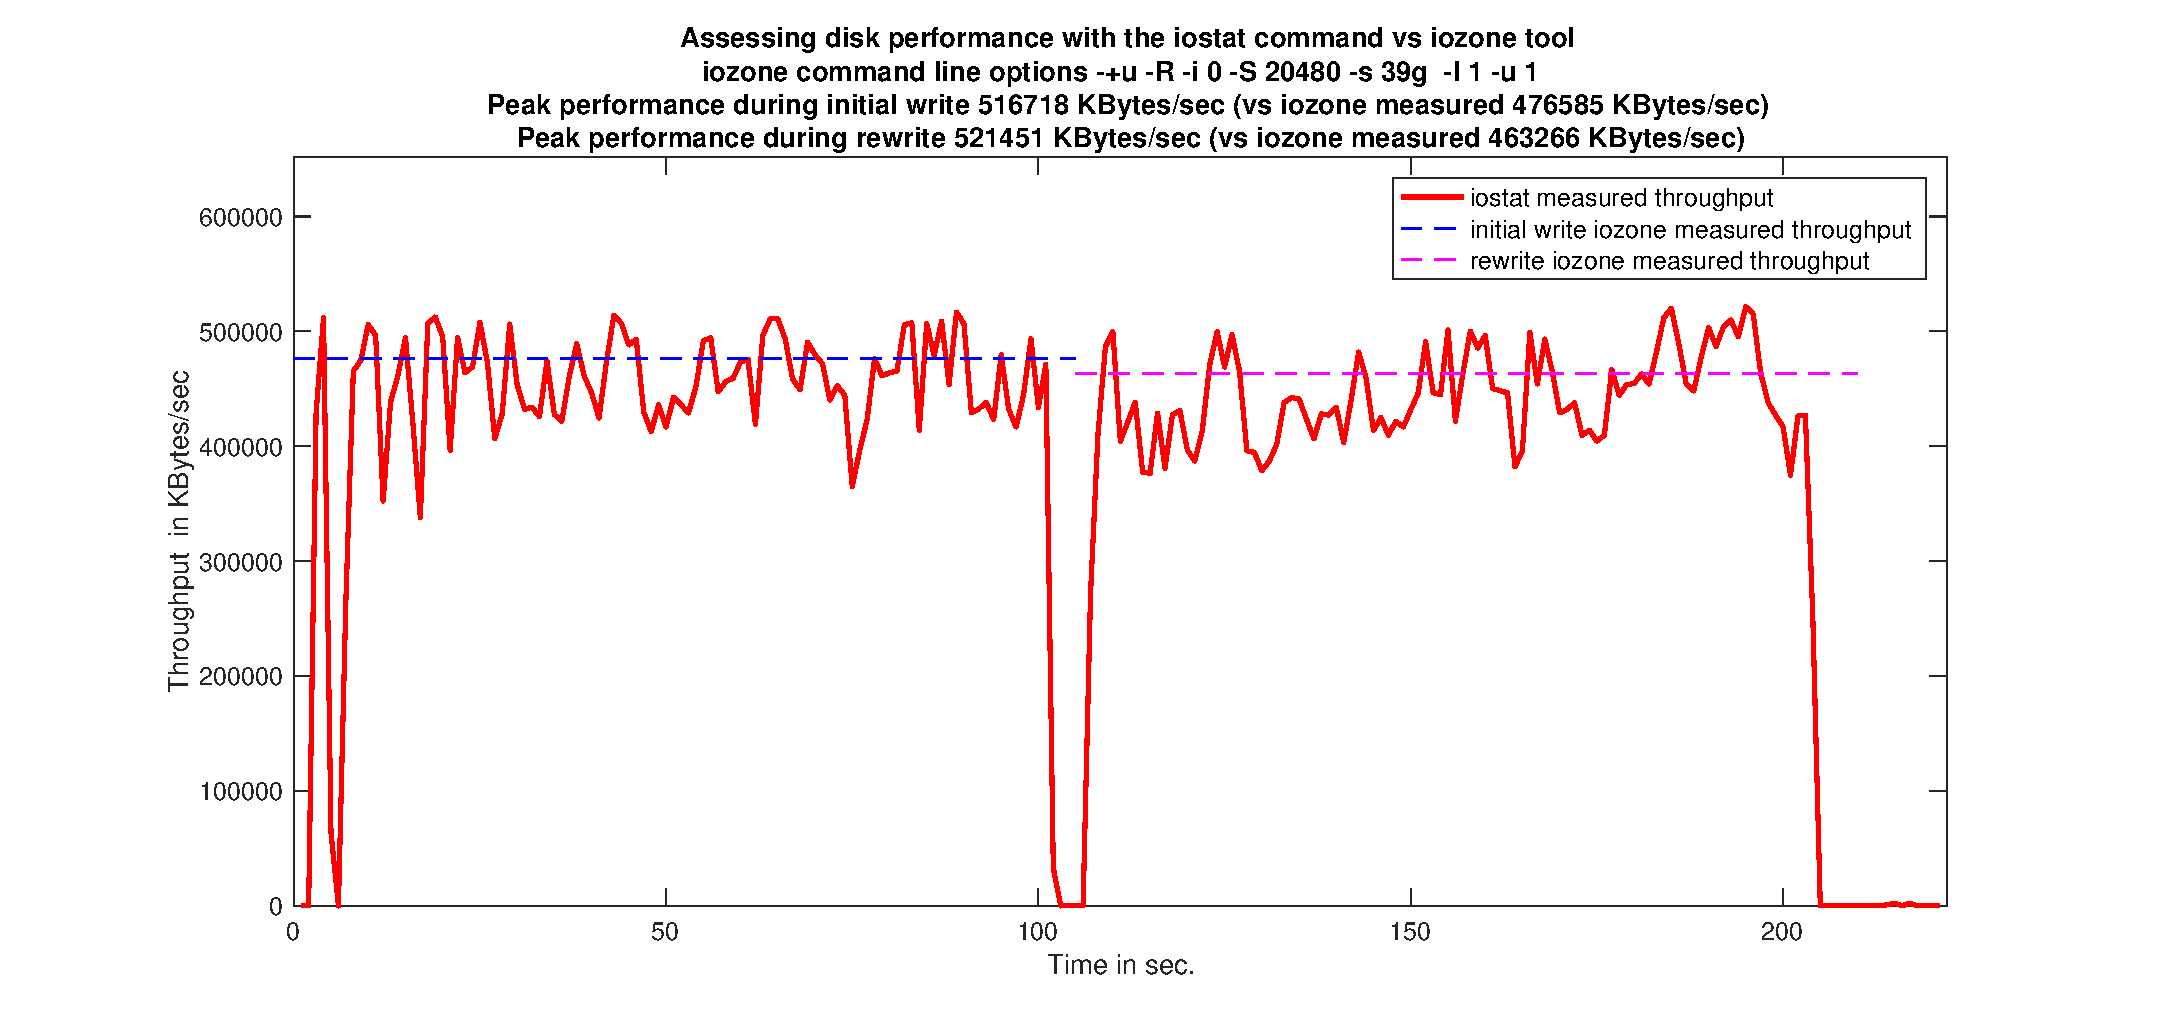
\includegraphics[width=1.1\columnwidth]{EPS/iostat.eps}
\caption{Relação de disk performance medida pela ferramenta \texbf{iostat} vs performance medida pela ferramenta \textbf{iozone}. Para command line options /opt/csw/bin/iozone -+u -R -i 0 -S 20480 -s 39g -b /export/home/a57816/ESC\_ACTIVE\_BENCHMARKING\_HOME/teste\_write.xls -l 1 -u 1
}
\label{fig:iostat}
\end{figure}

Tal como suspeitávamos existe alguma imprecisão nos valores apresentados pela ferramenta \textbf{iozone} vs os apresentados pela ferramente \textbf{iostat}. Como era previsível o peak throughput aconteceu na acção de rewrite (521451 KBytes/sec), através da medição da ferramenta \textbf{iostat}. Tal não se revelou verdade novamente nos valores apresentados pela ferramenta \textbf{iozone}. 
\par 
Façamos uma análise mais profunda das systems calls que a ferramenta \textbf{iozone} realiza para o cálculo dos resultados.

\subsection{Take 2 -- uma análise com truss}

Analisemos o tipo de system calls realizada pela ferramenta recorrendo ao seguinte comando \textbf{truss}:

\begin{lstlisting}[style=command]
truss -o truss_report_write.txt -df /opt/csw/bin/iozone -+u -R -i 0 -S 20480 -s 39g -b /export/home/a57816/ESC_ACTIVE_BENCHMARKING_HOME/teste_write.xls -l 1 -u 1 
\end{lstlisting}

Da análise do ficheiro truss\_report\_write.txt reparamos que o ficheiro de escrita do nosso interesse é o textbf{iozone.DUMMY.0} tal como confirmado pelo seguinte excerto: 
\begin{lstlisting}
...
...
9990:- 0.0986-open("iozone.DUMMY.0", O_RDWR|O_CREAT, 0640)--= 5
9989:- 0.0993-pollsys(0xFFFF80FFBFFFF8A0, 0, 0xFFFF80FFBFFFF920, 0x00000000) = 0
9989:- 0.0994-getpid()----------= 9989 [9988]
9990:- 0.1000-pollsys(0xFFFF80FFBFFFEE80, 0, 0xFFFF80FFBFFFEF00, 0x00000000) = 0
9990:- 0.1002-getrusage(0xFFFF80FFBFFFEEA0)-----= 0
9990:- 0.1004-write(5, " y y y y y y y y\0\0\0\0".., 4096)--= 4096
9990:- 0.1007-write(5, " y y y y y y y y\0\0\0\0".., 4096)--= 4096
9990:- 0.1010-write(5, " y y y y y y y y\0\0\0\0".., 4096)--= 4096
9990:- 0.1012-write(5, " y y y y y y y y\0\0\0\0".., 4096)--= 4096
9990:- 0.1015-write(5, " y y y y y y y y\0\0\0\0".., 4096)--= 4096
9990:- 0.1018-write(5, " y y y y y y y y\0\0\0\0".., 4096)--= 4096
9990:- 0.1020-write(5, " y y y y y y y y\0\0\0\0".., 4096)--= 4096
9990:- 0.1023-write(5, " y y y y y y y y\0\0\0\0".., 4096)--= 4096
9990:- 0.1025-write(5, " y y y y y y y y\0\0\0\0".., 4096)--= 4096
...
...
\end{lstlisting}

Podemos retirar dois aspectos importantes do seguinte excerto, sendo estes o \textbf{método de medição -- via getrusage\footnote{\url{http://linux.die.net/man/2/getrusage}}},  e o textbf{nome do ficheiro -- iozone.DUMMY.0} , o seu respectivo \textbf{descritor de ficheiro  -- 5}  e \textbf{ tamanho de record utilizado - 4096 bytes }.\par 
Podemos ainda analisar o momento do término da contagem do tempo para a operação de \texbf{initial write}. Um pouco para nosso espanto a medição do tempo é terminada antes da garantia de sincronização dos dados com disco (conferir linhas 10223827 e 10223828 do próximo excerto). Ou seja, este tipo de medição não será certamente o mais preciso uma vez que poderão ocorrer descrepâncias entre o tempo calculado pela ferramenta e o tempo real que a ferramenta demora a completar a operação de escrita e sincronização. \textbf{Encontramos a primeira imprecisão!}
\label{imprecisao}
\begin{lstlisting}
...
...
10223819 9990:-380.0682--write(5, " y y y y y y y y\0\0\0\0".., 4096)--= 4096
10223820 9990:-380.0683--write(5, " y y y y y y y y\0\0\0\0".., 4096)--= 4096
10223821 9990:-380.0683--write(5, " y y y y y y y y\0\0\0\0".., 4096)--= 4096
10223822 9990:-380.0683--write(5, " y y y y y y y y\0\0\0\0".., 4096)--= 4096
10223823 9990:-380.0684--write(5, " y y y y y y y y\0\0\0\0".., 4096)--= 4096
10223824 9990:-380.0684--write(5, " y y y y y y y y\0\0\0\0".., 4096)--= 4096
10223825 9990:-380.0684--write(5, " y y y y y y y y\0\0\0\0".., 4096)--= 4096
10223826 9990:-380.0685--write(5, " y y y y y y y y\0\0\0\0".., 4096)--= 4096
10223827 9990:-380.0685--getrusage(0xFFFF80FFBFFFEEA0)-----= 0
10223828 9990:-380.6926--fdsync(5, FSYNC)--------= 0
10223829 9990:-380.6928--close(5)----------= 0
10223830 9990:-380.6930--_exit(0)
...
...
\end{lstlisting}

Continuando a análise do ficheiro truss\_report\_write.txt reparamos que o ficheiro de escrita do nosso interesse continua a ser o textbf{iozone.DUMMY.0}.


\begin{lstlisting}
...
...
10223853 9992:-383.3986--open("iozone.DUMMY.0", O_RDWR)------= 5
10223854 9989:-383.3994--pollsys(0xFFFF80FFBFFFF8A0, 0, 0xFFFF80FFBFFFF920, 0x00000000) = 0
10223855 9989:-383.3996--getpid()----------= 9989 [9988]
10223856 9992:-383.4000--pollsys(0xFFFF80FFBFFFEE90, 0, 0xFFFF80FFBFFFEF10, 0x00000000) = 0
10223857 9992:-383.4002--getrusage(0xFFFF80FFBFFFEEB0)-----= 0
10223858 9992:-383.4004--getrusage(0xFFFF80FFBFFFEEB0)-----= 0
10223859 9992:-383.4007--write(5, " y y y y y y y y\0\0\0\0".., 4096)--= 4096
10223860 9992:-383.4010--write(5, " y y y y y y y y\0\0\0\0".., 4096)--= 4096
10223861 9992:-383.4013--write(5, " y y y y y y y y\0\0\0\0".., 4096)--= 4096
10223862 9992:-383.4016--write(5, " y y y y y y y y\0\0\0\0".., 4096)--= 4096
10223863 9992:-383.4018--write(5, " y y y y y y y y\0\0\0\0".., 4096)--= 4096
10223864 9992:-383.4021--write(5, " y y y y y y y y\0\0\0\0".., 4096)--= 4096
10223865 9992:-383.4023--write(5, " y y y y y y y y\0\0\0\0".., 4096)--= 4096
10223866 9992:-383.4026--write(5, " y y y y y y y y\0\0\0\0".., 4096)--= 4096
10223867 9992:-383.4028--write(5, " y y y y y y y y\0\0\0\0".., 4096)--= 4096
10223868 9992:-383.4031--write(5, " y y y y y y y y\0\0\0\0".., 4096)--= 4096
10223869 9992:-383.4034--write(5, " y y y y y y y y\0\0\0\0".., 4096)--= 4096
10223870 9992:-383.4036--write(5, " y y y y y y y y\0\0\0\0".., 4096)--= 4096
10223871 9992:-383.4039--write(5, " y y y y y y y y\0\0\0\0".., 4096)--= 4096
10223872 9992:-383.4042--write(5, " y y y y y y y y\0\0\0\0".., 4096)--= 4096
10223873 9992:-383.4044--write(5, " y y y y y y y y\0\0\0\0".., 4096)--= 4096
...
...
\end{lstlisting}
\newpage
\subsection{Take 3 -- uma análise com dtrace}

Deste padrão de open() , write(), e read() podemos criar um ficheiro dtrace que calcule o tempo entre as syscalls open() e close() com o descritor de ficheiro = 5, e calcular o total de bytes escrito pelas syscalls write() entre open() e close().

\begin{lstlisting}
#!/usr/sbin/dtrace -s

#pragma D option quiet

syscall::open*:entry
{
  self->pathname = copyinstr(arg1); 
}

syscall::open*:return
/strstr(self->pathname,"iozone.DUMMY.0") != NULL /
{
  self->start = timestamp; 
  total_size = 0;
}

fsinfo:::write 
/strstr(args[0]->fi_pathname,"iozone.DUMMY.0") != NULL /
{
  kb = arg1 / 1024;
  total_size = total_size + kb ; 
}

syscall::close*:return
/total_size > 0 && self->start /
{
  self->stop_t = timestamp; 
  printf("\n\n###############################################\n");
  printf("total time: %d\n", self->stop_t - self->start );
  printf("total size: %d\n", total_size);
  printf("###############################################\n\n");
  total_size = 0;
}
\end{lstlisting}

Ora, a execução do script dtrace e ferramenta iozone resultou no seguinte output:

\begin{lstlisting}
	Iozone: Performance Test of File I/O
	        Version $Revision: 3.434 $
		Compiled for 64 bit mode.
		Build: Solaris10 

	Contributors:William Norcott, Don Capps, Isom Crawford, Kirby Collins
	             Al Slater, Scott Rhine, Mike Wisner, Ken Goss
	             Steve Landherr, Brad Smith, Mark Kelly, Dr. Alain CYR,
	             Randy Dunlap, Mark Montague, Dan Million, Gavin Brebner,
	             Jean-Marc Zucconi, Jeff Blomberg, Benny Halevy, Dave Boone,
	             Erik Habbinga, Kris Strecker, Walter Wong, Joshua Root,
	             Fabrice Bacchella, Zhenghua Xue, Qin Li, Darren Sawyer,
	             Vangel Bojaxhi, Ben England, Vikentsi Lapa,
	             Alexey Skidanov.

	Run began: Tue Apr 19 03:18:52 2016

	CPU utilization Resolution = 0.000 seconds.
	CPU utilization Excel chart enabled
	Excel chart generation enabled
	File size set to 40894464 kB
	Command line used: /opt/csw/bin/iozone -+u -R -i 0 -S 20480 -s 39g -b /export/home/a57816/ESC_ACTIVE_BENCHMARKING_HOME/teste_write.xls -l 1 -u 1
	Output is in kBytes/sec
	Time Resolution = 0.000001 seconds.
	Processor cache size set to 20480 kBytes.
	Processor cache line size set to 32 bytes.
	File stride size set to 17 * record size.
	Min process = 1 
	Max process = 1 
	Throughput test with 1 process
	Each process writes a 40894464 kByte file in 4 kByte records

	Children see throughput for  1 initial writers 	=  326724.00 kB/sec
	Parent sees throughput for  1 initial writers 	=  309091.96 kB/sec
	Min throughput per process 			=  326724.00 kB/sec 
	Max throughput per process 			=  326724.00 kB/sec
	Avg throughput per process 			=  326724.00 kB/sec
	Min xfer 					= 40894464.00 kB
	CPU Utilization: Wall time  125.165    CPU time  125.165    CPU utilization 100.00 %



###############################################
total time: 132303544264
total size: 40894464
###############################################


	Children see throughput for  1 rewriters 	=  338724.72 kB/sec
	Parent sees throughput for  1 rewriters 	=  320792.40 kB/sec
	Min throughput per process 			=  338724.72 kB/sec 
	Max throughput per process 			=  338724.72 kB/sec
	Avg throughput per process 			=  338724.72 kB/sec
	Min xfer 					= 40894464.00 kB
	CPU utilization: Wall time  120.731    CPU time  120.730    CPU utilization 100.00 %



###############################################
total time: 127477939460
total size: 40894464
###############################################




"Throughput report Y-axis is type of test X-axis is number of processes"
"Record size = 4 kBytes "
"Output is in kBytes/sec"

"  Initial write "  326724.00 

"        Rewrite "  338724.72 


"CPU utilization report Y-axis is type of test X-axis is number of processes"
"Record size = 4 kBytes "
"Output is in CPU%"

"  Initial write "     100.00 

"        Rewrite "     100.00 


iozone test complete.
\end{lstlisting}

Para o caso de initial write o script dtrace calculou 132303544264 nano-segundos como o tempo necessário à escrita -- equivalente a 132.30 segundos. Encontramos já neste valor uma pequena descrepância versus os 125.165 segundos de Wall time apresentados pela ferramenta iozone. Analisemos o throughput médio calculado: 40894464 KB / 132.30 seg = 309104.036 KB/sec, também este diferente dos 326724.00 KB/sec calculados pela ferramenta iozone. \par 
Procedendo de igual forma para re-write temos como tempo calculado pelo script dtrace 127477939460 nano-segundos como o tempo necessário à re-escrita -- equivalente a 127.477 segundos.  
Encontramos novamente  uma pequena descrepância versus os 120.731 segundos de Wall time apresentados pela ferramenta iozone. Analisemos o throughput médio calculado: 40894464 KB / 127.477 seg = 320798.763 KB/sec , também este diferente dos 338724.72 KB/sec calculados pela ferramenta iozone. \par
De um modo constante a ferramenta iozone foi mais "otimista" nos valores medidos, e acreditamos que a \textbf{diferença de valores obtidos se prende com a imprecisão que detectamos anteriormente na secção \ref{imprecisao}}.
\newpage
\section{Trabalho Futuro}

\epigraph{
Running a benchmark is the easy part. Understanding a benchmark can take much longer.
\vspace{3mm}\\ \url{http://www.brendangregg.com/ActiveBenchmarking/bonnie++.html}}\par 




Tal como mencionado em trabalhos anteriores a ferramenta DTrace mostra-se bastante útil e única em termos de funcionalidades quando necessitamos de agregar informação de vários processos/threads,etc. Contudo, esta representa uma pequena porção de todo o trabalho de análise e tratamento de dados necessário para a validação de valores apresentados por ferramentas de benchmarking como o caso da iozone. Sem a análise anterior via \textbf{iostat} e \textbf{truss} seria impossível tirar qualquer tipo de conclusão.\par
Ora, o trabalho futuro prende-se com o teste de outras funcionalidades da ferramenta iozone corroborando/desmentindo os valores nela anunciados.
Por vezes, durante o processo de compreensão da ferramenta iozone foi necessário analisar instrução-a-instrução resultante, com algumas descobertas interessantes.
\par 
Retratamos sobretudo a capacidade analisar funcionalidades disponibilizadas e a sua correta aplicação na resolução de problemas de computação tendo sempre em conta o mínimo de alteração possível na medição de perfomance do sistema analisado.



\end{document}


